\documentclass[onecolumn]{IEEEtran}

\usepackage{amsmath}
\usepackage[spanish]{babel}
\usepackage[colorlinks=true, urlcolor=blue]{hyperref}
\usepackage{graphicx}
\usepackage{titlesec}
\usepackage{titling}

\titleformat{\section}
{\Large}
{}
{0cm}
{}[\titlerule]

\title{An\'alisis de regresi\'on sobre la relaci\'on de las estad\'isticas de MPG y PPG en partidos de postemporada de la NBA}
\author{Rudy Miranda Bastias\\
    Github (scripts): \url{https://github.com/SolaireLordOfSunlight/Linear-Regression}
}
\date{Abril, 2023}

\begin{document}
    \maketitle

    \section{Introducci\'on}
    Se busca confirmar si la relaci\'on entre la cantidad de puntos anotados por un jugador de la NBA, frente a la cantidad de minutos jugados por partido tienen una relaci\'on del tipo lineal.

    Los datos corresponden a los playoff (post-temporada) de la temporada 2021-22 de la NBA obtenidos de su sitio web oficial.

    Un punto a enfatizar es que las 79 unidades de  observaci\'on son jugadores de la misma posici\'on, donde se toma en cuenta su promedio de puntos por partidos (PPG) y su promedio de minutos por partido (MPG).

    \begin{figure}[h]
       \centering
       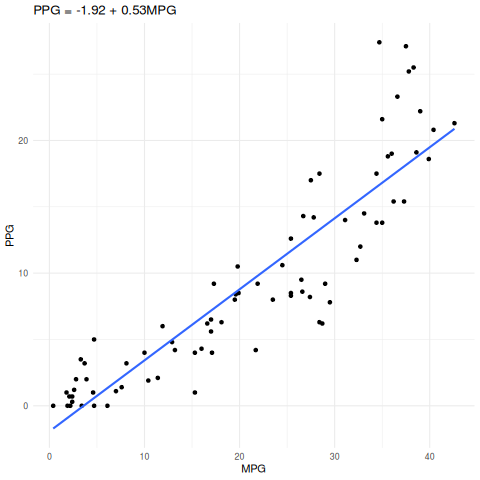
\includegraphics[width=0.5\textwidth]{../plot1.png}
    \end{figure}

    \section{Modelo Poblacional}
    
    \begin{equation}
        PPG = \beta_0 + \beta_1 MPG + \varepsilon        
    \end{equation}
    
    \section{Estimaci\'on de Parametros}
    \subsection*{Comandos \textit{R}}
    \begin{verbatim}
table_values <- read.csv("./nba_stats.csv")
(summary(lm(formula = PPG ~ MPG, data = table_values)))
    \end{verbatim}
    \newpage
    \subsection*{Resultados}
    \begin{table}[h]
        \centering
        \begin{tabular}{l l c c r}
            & & $\hat{\beta_0}$ & $\hat{\beta_1}$ & \quad $R^2 = 0.8037$ \\
            PPG & = & -1.92 & 0.53 &\\
            $s.e$ &  & 0.73 & 0.03 &\\
            $t$ & & -2.65 & 17.9 &\\
            valor-$p$ & & 0.01 & $\approx$ 0 &
        \end{tabular}
    \end{table}
    
    Aqui el $\hat{\beta_1}$ indica que los jugadores en promedio anotan 0.53 por cada minuto jugado. Por otro lado $\hat{\beta_0} = -1.92$ es un numero que no tiene sentido en la realidad, seria buena idea quitar el intercepto.

    Interpretando $R^2$, el 80\% de la variaci\'on de la estad\'istica $PPG$ se explica por la de $MPG$.
    %\section{Modelo Estimado}
    %
    %\begin{equation}
    %    PPG = \hat{\beta_0} + \hat{\beta_1} MPG + \varepsilon        
    %\end{equation}
    \section{Validaci\'on del Modelo}
    Proponemos las hip\'otesis
    
    $$
        H_0 : \beta_1 = 0
    $$
    $$
        H_1 : \beta_1 \neq 0
    $$

    rechazando $H_0$ dado el valor-$p \approx 0$ del resumen anterior.

    \section{An\'alisis de Residuos}
    \begin{figure}[ht]
        \centering
       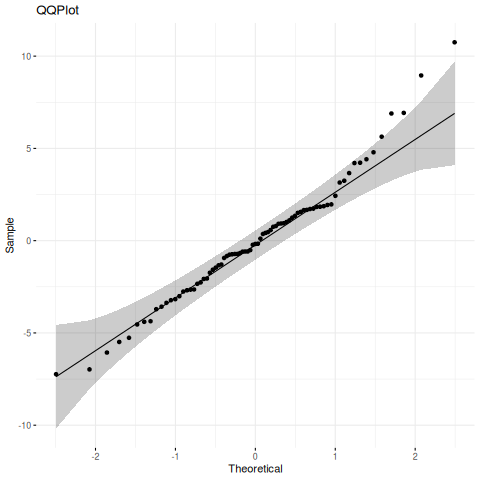
\includegraphics[width=0.5\textwidth]{../plot2.png}
    \end{figure}
    Una hip\'otesis que deben cumplir nuestro modelo es que $\varepsilon_i = (Y_i - \bar{Y}) \sim N(0, \sigma^2)$

    Aplicando distintos test de normalidad, tanto parametricos como no parametricos
    
    \begin{table}[h]
        \begin{center}
            \begin{tabular}{|c|c|}
                \hline Test & Valor P \\ \hline
                Jarque-Bera & 0.04469 \\ \hline
                Kolmogorov-Smirnov & 3.847e-05\\ \hline
                Shapiro-Wilk & 0.1174 \\ \hline
                Anderson-Darling & 0.1493 \\ \hline
            \end{tabular}
        \end{center}
    \end{table}

    Con un nivel de significancia de 0.05, podriamos considerar la distribuci\'on como una normal.

    Ahora, al hacer un test de hip\'otesis con el comando \textit{t.test} sobre la media con la hip\'otesis nula $H_0: \mu = 0$ obtenemos un valor $p = 1$, con lo que aceptamos $H_0$.

    Con ello se cumplen los dos supuestos de la distribuci\'on de los residuos.

    \subsection{Independencia de los Residuos}

    Aplicando el test de Durbin-Watson, con las siguientes hip\'otesis
    
    $$
        H_0\text{ : los errores son independientes}
    $$
    $$
        H_1\text{ : los errores no son independientes}
    $$

    Aceptamos la hip\'otesis nula, puesto que el valor-$p = 0.21 > 0.05$ el nivel de significancia con el cual trabajamos en este informe. 

    Referencia: \url{https://fhernanb.github.io/libro_regresion/indep.html}

    \section{Conclusi\'on}
    Es clara la relaci\'on entre los minutos jugados y los puntos anotados, pero seria una buena desici\'on incluir mas variables a este modelo en vez de solo dejarlo en dos, y como se dijo anteriormente podriamos quitar el intercepto de nuestra funci\'on de regresi\'on poblacional.

\end{document}
